\section{Pseudo-dielectric inversion on gold}

The previous example exposed the bias that a thin overlayer imprints on
the pseudo-dielectric inversion. The final benchmark runs the same
inversion on a bare metallic substrate, where by construction there is
no overlayer and the closed-form result must return the input index
exactly across the full wavelength range. The substrate is gold,
tabulated in the Johnson--Christy table at the ten wavelengths
\SIlist{400;450;500;550;600;650;700;800;900;1000}{\nano\metre} and
linearly interpolated on a 601-point grid between \SI{400}{\nano\metre}
and \SI{1000}{\nano\metre}. The stack is reduced to the two
half-spaces air\,/\,Au (empty thickness list), and the angle of incidence
is fixed at $\theta_0 = \SI{70}{\degree}$.

The TMM returns the complex amplitudes $r_s$ and $r_p$ directly, from
which the ellipsometric ratio $\rho = r_p/r_s$ is formed, negated to
match the sign convention of the Azzam--Bashara / Aspnes pseudo-dielectric
inversion, and fed into
\begin{equation}
  \langle\varepsilon\rangle = \sin^{2}\theta_0\left[1 + \tan^{2}\theta_0\left(\frac{1-\rho}{1+\rho}\right)^{2}\right]. \label{eq:gold-pseudoeps}
\end{equation}
For a bare substrate of complex index $N = n + \ii k$ the inversion is
exact,
\begin{equation}
  \langle\varepsilon\rangle(\lambda) = N^{2}(\lambda),\qquad N = \sqrt{\langle\varepsilon\rangle}, \label{eq:gold-N}
\end{equation}
on the branch $\Imy(N) \ge 0$ for a passive absorber. Panel (a) compares
$n(\lambda)$ and $k(\lambda)$ extracted from $\sqrt{\langle\varepsilon\rangle}$
against the input Johnson--Christy values; panel (b) shows the same
comparison for the real and imaginary parts of $\varepsilon$ directly.

\begin{center}
\begin{tikzpicture}
  \fill[black!4]   (0, 0) rectangle (5, 1.6);
  \fill[yellow!45] (0,-1.2) rectangle (5, 0);
  \draw[thick] (0,0) -- (5,0);
  \node[lbl, anchor=east] at (4.9, 1.2) {air};
  \node[lbl, anchor=east] at (4.9,-0.7) {Au};
  \raysketch{1.6}{55}{f}
\end{tikzpicture}
\end{center}

\begin{figure}[!htbp]
  \centering
  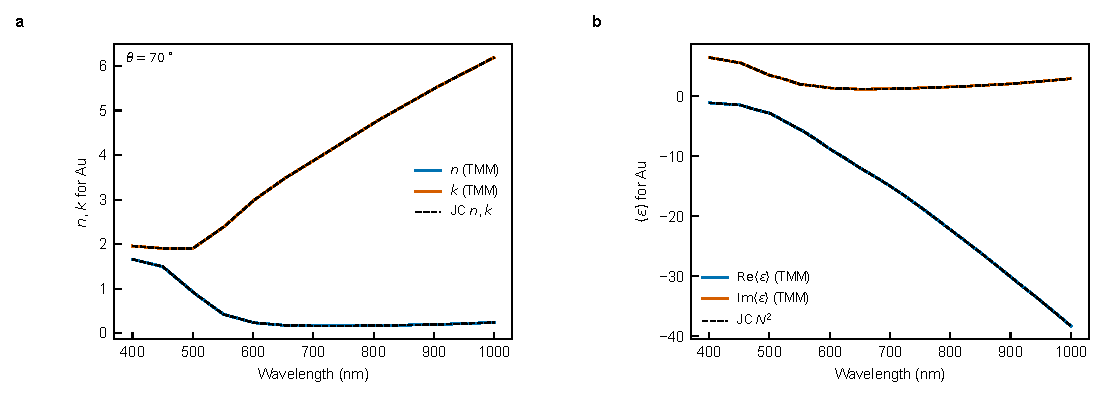
\includegraphics[width=\textwidth]{16_gold_ellipsometry.pdf}
  \caption{(a) $n(\lambda), k(\lambda)$ and (b) $\Rey\varepsilon, \Imy\varepsilon$ from the Johnson--Christy table (dashed) against the TMM-inverted pseudo-dielectric function from equation~\eqref{eq:gold-pseudoeps} (solid).}
  \label{fig:gold}
\end{figure}

Recovering $N$ via $\sqrt{\langle\varepsilon\rangle}$ reproduces the input
Johnson--Christy data to $\max|\Delta N| \approx \num{1e-14}$ over the
full wavelength window. Equation~\eqref{eq:gold-N} is therefore satisfied
end-to-end: the TMM returns $r_s$ and $r_p$ at machine precision, the
ratio $\rho$ inherits that precision, and the closed-form
inversion~\eqref{eq:gold-pseudoeps} completes the round-trip without loss.
Taken together with the overlayer result of the previous section, this
example delimits the range over which the pseudo-dielectric function is
an exact inverse and the range over which it functions as a
thickness-biased effective quantity.


